% TODO: 
% check again if the text are smooth enough from paragraph or from sub points to another sub points (Check the ChatGPT under "Hausarbeit überarbeiten unerquicklich")

\documentclass[runningheads]{res/llncs}

\usepackage[T1]{fontenc}
\usepackage[utf8]{inputenc}
\usepackage[ngerman]{babel}
\usepackage{graphicx}
\usepackage{subcaption}
\usepackage{float}
\usepackage{tabularx}
\usepackage{booktabs}
\usepackage{url}
% Makes citations, URLs, table of contents entries and cross-references clickable in the PDF.
% Use hidelinks for a clean academic style without colored boxes.
\usepackage{hyperref}
\usepackage[acronym,nonumberlist,section=section]{glossaries}
% Sortierung durch LaTeX; kein separater makeglossaries-Aufruf erforderlich.
\makenoidxglossaries
% Zentrale Definitionen des Abkürzungsverzeichnisses.
% Im Haupttext: \gls{etcs} (erste Verwendung ausgeschrieben),
% \acrshort{etcs} (nur Abkürzung), \acrlong{etcs} (nur Langform).
% Neue Einträge werden automatisch im Verzeichnis aufgeführt.

\newacronym[description={Zweite Mobilfunkgeneration (\textit{Second Generation})},sort={2g}]{2g}{2G}{Zweite Mobilfunkgeneration (\textit{Second Generation})}
\newacronym[description={\textit{Triple Data Encryption Standard}; dreifache Anwendung des DES-Verfahrens},sort={3des}]{3des}{3DES}{Triple Data Encryption Standard}
\newacronym[description={\textit{3rd Generation Partnership Project}; Standardisierungsgremium für Mobilfunksysteme},sort={3gpp}]{3gpp}{3GPP}{3rd Generation Partnership Project}
\newacronym[description={Fünfte Mobilfunkgeneration (\textit{Fifth Generation})},sort={5g}]{5g}{5G}{Fünfte Mobilfunkgeneration (\textit{Fifth Generation})}
\newacronym[description={Sechste Mobilfunkgeneration (\textit{Sixth Generation})},sort={6g}]{6g}{6G}{Sechste Mobilfunkgeneration (\textit{Sixth Generation})}
\newacronym[description={Verschlüsselungsalgorithmen der GSM-Funkschnittstelle},sort={a51}]{a51}{A5/1}{Verschlüsselungsalgorithmen der GSM-Funkschnittstelle}
\newacronym[description={Verschlüsselungsalgorithmen der GSM-Funkschnittstelle},sort={a53}]{a53}{A5/3}{Verschlüsselungsalgorithmen der GSM-Funkschnittstelle}
\newacronym[description={\textit{Automatic Train Control}; automatische Zugsteuerung},sort={atc}]{atc}{ATC}{Automatic Train Control}
\newacronym[description={\textit{Advanced Train Administration and Communications System}; funkbasiertes Zugsteuerungssystem von JR East},sort={atacs}]{atacs}{ATACS}{Advanced Train Administration and Communications System}
\newacronym[description={\textit{Automatic Train Operation}; automatisierter Zugbetrieb},sort={ato}]{ato}{ATO}{Automatic Train Operation}
\newacronym[description={\textit{Balise Transmission Module}; fahrzeugseitiges Modul zum Empfang von Eurobalisen-Telegrammen},sort={btm}]{btm}{BTM}{Balise Transmission Module}
\newacronym[description={\textit{Base Transceiver Station}; Basisstation eines Mobilfunknetzes},sort={bts}]{bts}{BTS}{Base Transceiver Station}
\newacronym[description={\textit{Cipher Block Chaining}; Betriebsart einer Blockchiffre},sort={cbc}]{cbc}{CBC}{Cipher Block Chaining}
\newacronym[description={\textit{Communications-Based Train Control}; kommunikationsbasierte Zugsteuerung},sort={cbtc}]{cbtc}{CBTC}{Communications-Based Train Control}
\newacronym[description={\textit{Control-Command and Signalling}; Zugsteuerung, Zugsicherung und Signalgebung},sort={ccs}]{ccs}{CCS}{Control-Command and Signalling}
\newacronym[description={\textit{Cryptography Research and Evaluation Committees}; japanisches Gremium zur Bewertung kryptographischer Verfahren},sort={cryptrec}]{cryptrec}{CRYPTREC}{Cryptography Research and Evaluation Committees}
\newacronym[description={\textit{Digital Automatic Train Control}; digitale Ausprägung der automatischen Zugsteuerung},sort={d-atc}]{d-atc}{D-ATC}{Digital Automatic Train Control}
\newacronym[description={\textit{Data Encryption Standard}; älterer symmetrischer Verschlüsselungsalgorithmus},sort={des}]{des}{DES}{Data Encryption Standard}
\newacronym[description={\textit{Driver Machine Interface}; Anzeige- und Bedienschnittstelle im Führerraum},sort={dmi}]{dmi}{DMI}{Driver Machine Interface}
\newacronym[description={\textit{European Rail Traffic Management System}; europäischer Rahmen für interoperable Zugsteuerung und Signalgebung},sort={ertms}]{ertms}{ERTMS}{European Rail Traffic Management System}
\newacronym[description={\textit{European Train Control System}; europäisches Zugsteuerungs- und Zugsicherungssystem innerhalb von ERTMS},sort={etcs}]{etcs}{ETCS}{European Train Control System}
\newacronym[description={\textit{European Vital Computer}; sicherheitskritischer ETCS-Fahrzeugrechner},sort={evc}]{evc}{EVC}{European Vital Computer}
\newacronym[description={\textit{Future Railway Mobile Communication System}; Nachfolgesystem von GSM-R},sort={frmcs}]{frmcs}{FRMCS}{Future Railway Mobile Communication System}
\newacronym[description={\textit{Grade of Automation 4}; vollautomatischer, unbegleiteter Zugbetrieb},sort={goa4}]{goa4}{GoA4}{Grade of Automation 4}
\newacronym[description={\textit{Global System for Mobile Communications -- Railway}; eisenbahnspezifisches Mobilfunksystem},sort={gsm-r}]{gsm-r}{GSM-R}{Global System for Mobile Communications -- Railway}
\newacronym[description={\textit{Home Location Register}; zentrale Teilnehmerdatenbank eines GSM-Netzes},sort={hlr}]{hlr}{HLR}{Home Location Register}
\newacronym[description={\textit{Hash-based Message Authentication Code} auf Basis von SHA-256},sort={hmac-sha256}]{hmac-sha256}{HMAC-SHA256}{\textit{Hash-based Message Authentication Code} auf Basis von SHA-256}
\newacronym[description={\textit{Intrusion Detection System}; System zur Angriffserkennung},sort={ids}]{ids}{IDS}{Intrusion Detection System}
\newacronym[description={\textit{International Electrotechnical Commission}; internationale elektrotechnische Normungsorganisation},sort={iec}]{iec}{IEC}{International Electrotechnical Commission}
\newacronym[description={\textit{Internet Protocol}; Netzwerkprotokoll für paketvermittelte Kommunikation},sort={ip}]{ip}{IP}{Internet Protocol}
\newacronym[description={\textit{International Organization for Standardization}; internationale Normungsorganisation},sort={iso}]{iso}{ISO}{International Organization for Standardization}
\newacronym[description={Informationstechnik},sort={it}]{it}{IT}{Informationstechnik}
\newacronym[description={\textit{Japanese National Railways}; frühere staatliche japanische Eisenbahngesellschaft},sort={jnr}]{jnr}{JNR}{Japanese National Railways}
\newacronym[description={\textit{Japan Railways}; Gruppe der aus der JNR hervorgegangenen Eisenbahnunternehmen},sort={jr}]{jr}{JR}{Japan Railways}
\newacronym[description={Symmetrischer EuroRadio-Schlüssel zur Bildung eines \textit{Message Authentication Code}},sort={kmac}]{kmac}{KMAC}{Symmetrischer EuroRadio-Schlüssel zur Bildung eines \textit{Message Authentication Code}}
\newacronym[description={\textit{Key Management Centre}; Stelle zur Verwaltung und Verteilung kryptographischer Schlüssel},sort={kmc}]{kmc}{KMC}{Key Management Centre}
\newacronym[description={\textit{Key Management System}; System zur Verwaltung kryptographischer Schlüssel},sort={kms}]{kms}{KMS}{Key Management System}
\newacronym[description={\textit{ETCS Level 2 without Signals}; ETCS Level 2 ohne ortsfeste Lichtsignale},sort={l2os}]{l2os}{L2oS}{ETCS Level 2 without Signals}
\newacronym[description={\textit{Leaky Coaxial Cable}; Schlitz- beziehungsweise Leckkabel zur Funkversorgung entlang der Strecke},sort={lcx}]{lcx}{LCX}{Leaky Coaxial Cable}
\newacronym[description={\textit{Lineside Electronic Unit}; streckenseitige elektronische Einheit zur Ansteuerung von Eurobalisen},sort={leu}]{leu}{LEU}{Lineside Electronic Unit}
\newacronym[description={Leit- und Sicherungstechnik},sort={lst}]{lst}{LST}{Leit- und Sicherungstechnik}
\newacronym[description={\textit{Movement Authority}; ETCS-Fahrterlaubnis},sort={ma}]{ma}{MA}{Movement Authority}
\newacronym[description={\textit{Message Authentication Code}; kryptographischer Prüfwert für Integrität und Authentizität einer Nachricht},sort={mac}]{mac}{MAC}{Message Authentication Code}
\newacronym[description={\textit{Mission-Critical Services}; 3GPP-Dienste für missionskritische Kommunikation},sort={mcx}]{mcx}{MCx}{Mission-Critical Services}
\newacronym[description={\textit{Multiple Independent Levels of Security}; Architekturprinzip zur strikten Isolation von Systempartitionen},sort={mils}]{mils}{MILS}{Multiple Independent Levels of Security}
\newacronym[description={\textit{Moving Target Defense}; dynamische Veränderung von Systemparametern zur Erschwerung von Angriffen},sort={mtd}]{mtd}{MTD}{Moving Target Defense}
\newacronym[description={\textit{On-Board Unit}; fahrzeugseitige Steuerungs- und Kommunikationseinheit},sort={obu}]{obu}{OBU}{On-Board Unit}
\newacronym[description={\textit{Public Key Infrastructure}; Infrastruktur zur Verwaltung digitaler Zertifikate und Schlüssel},sort={pki}]{pki}{PKI}{Public Key Infrastructure}
\newacronym[description={\textit{Reliability, Availability, Maintainability and Safety}; Zuverlässigkeit, Verfügbarkeit, Instandhaltbarkeit und Sicherheit},sort={rams}]{rams}{RAMS}{Reliability, Availability, Maintainability and Safety}
\newacronym[description={\textit{Radio Block Centre}; ETCS-Streckenzentrale zur Erzeugung und Übertragung von Fahrterlaubnissen},sort={rbc}]{rbc}{RBC}{Radio Block Centre}
\newacronym[description={\textit{Railway Mobile Radio}; UIC-Rahmen für den zukünftigen Bahnmobilfunk},sort={rmr}]{rmr}{RMR}{Railway Mobile Radio}
\newacronym[description={\textit{Rail Radio Intrusion Detection System}; Angriffserkennungssystem für CBTC-Funkkommunikation},sort={rrids}]{rrids}{RRIDS}{Rail Radio Intrusion Detection System}
\newacronym[description={\textit{Railway Technical Research Institute}; japanisches Eisenbahnforschungsinstitut},sort={rtri}]{rtri}{RTRI}{Railway Technical Research Institute}
\newacronym[description={\textit{Safety-Critical Application Development Environment}; Entwicklungsumgebung für sicherheitskritische Software},sort={scade}]{scade}{SCADE}{Safety-Critical Application Development Environment}
\newacronym[description={\textit{Secure Hash Algorithm} mit einer Ausgabelänge von 256 Bit},sort={sha-256}]{sha-256}{SHA-256}{\textit{Secure Hash Algorithm} mit einer Ausgabelänge von 256 Bit}
\newacronym[description={\textit{Single Point of Failure}; einzelne Fehlerstelle, deren Ausfall das Gesamtsystem beeinträchtigen kann},sort={spof}]{spof}{SPOF}{Single Point of Failure}
\newacronym[description={\textit{Transmission Control Protocol/Internet Protocol}; grundlegende Protokollfamilie IP-basierter Netze},sort={tcpip}]{tcpip}{TCP/IP}{Transmission Control Protocol/Internet Protocol}
\newacronym[description={\textit{Time Division Multiple Access}; Zeitmultiplexverfahren für den gemeinsamen Zugriff auf einen Funkkanal},sort={tdma}]{tdma}{TDMA}{Time Division Multiple Access}
\newacronym[description={\textit{Train Integrity Monitoring System}; System zur Überwachung der Vollständigkeit eines Zuges},sort={tims}]{tims}{TIMS}{Train Integrity Monitoring System}
\newacronym[description={\textit{Transport Layer Security}; Protokoll zur kryptographischen Absicherung von Netzwerkverbindungen},sort={tls}]{tls}{TLS}{Transport Layer Security}
\newacronym[description={\textit{Telecom On-Board Architecture}; modulare fahrzeugseitige Telekommunikationsarchitektur},sort={toba}]{toba}{TOBA}{Telecom On-Board Architecture}
\newacronym[description={\textit{Train Real-Time Data Protocol}; Kommunikationsprotokoll für Zugnetzwerke},sort={trdp}]{trdp}{TRDP}{Train Real-Time Data Protocol}
\newacronym[description={\textit{Technical Specification for Interoperability relating to Control-Command and Signalling}; europäische Interoperabilitätsspezifikation für Zugsteuerung, Zugsicherung und Signalgebung},sort={tsiccs}]{tsiccs}{TSI CCS}{Technical Specification for Interoperability relating to Control-Command and Signalling}
\newacronym[description={\textit{International Union of Railways} (\textit{Union Internationale des Chemins de fer}); internationaler Eisenbahnverband},sort={uic}]{uic}{UIC}{\textit{International Union of Railways} (\textit{Union Internationale des Chemins de fer})}
\newacronym[description={Drahtlose lokale Netzwerktechnologie},sort={wi-fi}]{wi-fi}{Wi-Fi}{Drahtlose lokale Netzwerktechnologie}
\newacronym[description={Standard für digitale Zertifikate in Public-Key-Infrastrukturen},sort={x509}]{x509}{X.509}{Standard für digitale Zertifikate in Public-Key-Infrastrukturen}
\newacronym[description={\textit{Micro Timed Efficient Stream Loss-tolerant Authentication}; Verfahren zur zeitverzögerten Authentifizierung von Broadcast-Nachrichten},sort={mutesla}]{mutesla}{$\mu$TESLA}{Micro Timed Efficient Stream Loss-tolerant Authentication}
\newacronym[description={\textit{Wireless Local Area Network}; drahtloses lokales Netzwerk},sort={wlan}]{wlan}{WLAN}{Wireless Local Area Network}

\usepackage[backend=biber,style=alphabetic]{biblatex}
\addbibresource{reference.bib}
\addbibresource{Train_ITSec.bib}
\begin{document}
% Langformen sind im Text bereits ausgeschrieben; Abkürzungen bleiben kurz und verlinkt.
\glsunsetall


\title{Kommunikationssicherheit zwischen Zügen und Leitstellen: Eine vergleichende Untersuchung europäischer und japanischer Eisenbahnsysteme}

\titlerunning{Eisenbahn-Kommunikationssicherheit: Europa und Japan}

\author{Agha Muhammad Aslam -- \today}

% \date{\today}

\institute{
Hochschule Fulda \\
Fachbereich Angewandte Informatik \\
\email{agha-muhammad.aslam@informatik.hs-fulda.de}
}

\maketitle

\begin{abstract}
Die zunehmende Digitalisierung der Eisenbahn erhöht die Bedeutung sicherer Zug-Strecken-Kommunikation. Diese Hausarbeit untersucht anhand einer strukturierten Literaturanalyse, wie europäische und japanische Eisenbahnsysteme sicherheitskritische Kommunikation schützen und welche Sicherheitsgrenzen bestehen bleiben. Betrachtet werden insbesondere \gls{ertms}/\gls{etcs}, \gls{gsm-r}, \textit{EuroRadio} und \gls{frmcs} sowie \gls{d-atc}, \gls{atacs} und aktuelle japanische Forschungsansätze. Der Vergleich zeigt unterschiedliche Standardisierungsmodelle, zugleich aber eine gemeinsame Entwicklung hin zur stärkeren Entkopplung sicherheitskritischer Steuerungsfunktionen vom Übertragungsmedium. Kryptographische Verfahren schützen insbesondere Integrität und Authentizität, während die Verfügbarkeit der Kommunikation eine zentrale verbleibende Sicherheitsgrenze darstellt.

\keywords{Eisenbahnsicherheit \and \gls{etcs} \and \gls{ertms} \and \gls{gsm-r} \and \gls{frmcs} \and \gls{atacs} \and \gls{iec} 62280 \and Kommunikationssicherheit}
\end{abstract}

\section{Einleitung und Hintergrund}
\label{sec:Einleitung_und_Hintergrund}

Schienennetze bilden eine gesellschaftlich und wirtschaftlich bedeutsame Verkehrsinfrastruktur, deren zuverlässiger Betrieb Personen- und Güterverkehr sowie die öffentliche Sicherheit betrifft~\parencite[S. 4]{xiangliuCyber2020}. Mit zunehmender Digitalisierung hängt der Bahnbetrieb stärker von Informations-, Leit-, Sicherungs- und Kommunikationssystemen ab~\parencite[S. 3–4]{xiangliuCyber2020}. Fahrzeuge, streckenseitige Einrichtungen und betriebliche Zentralen tauschen dabei unter anderem Fahrterlaubnisse, Positions- und Geschwindigkeitsdaten aus, die unmittelbar zur Steuerung und Überwachung von Zugbewegungen dienen~\parencite[S. 88, 106, 163–166]{trinckaufETCS2024}. Störungen oder Manipulationen dieser Systeme können den Betrieb beeinträchtigen und im schlimmsten Fall die Betriebssicherheit gefährden~\parencite[S. 204, 207]{trinckaufETCS2024}. Entsprechend müssen Kommunikationsverbindungen sowohl gegen Fehler als auch gegen gezielte Angriffe geschützt werden~\parencite[S. 204]{trinckaufETCS2024}. 

Die bundesweite \gls{gsm-r}-Störung vom 23. Juni 2026 verdeutlicht diese Abhängigkeit: Nach dem Austausch eines \textit{Switches} verhinderte ein nicht gemeldeter Softwarefehler die automatische Aktivierung des redundanten Systems. Erst nach Ausschluss eines Cyberangriffs wurde nach rund 90 Minuten manuell auf die Rückfallebene umgeschaltet~\cite{dbinfragoUrsacheZugfunkStoerung2026}. Der Vorfall zeigt, dass neben dem Schutz vor Angriffen auch Redundanz, kontrollierte Wartungsprozesse und wirksames Störungsmanagement für die Sicherheit digitaler Bahnsysteme entscheidend sind.

Europa und Japan verfolgen unterschiedliche architektonische Ansätze. In Europa bildet \gls{ertms} einen interoperablen Rahmen zur Harmonisierung nationaler Signalsysteme und zur Unterstützung des grenzüberschreitenden Eisenbahnbetriebs~\cite{EuropeanCommission_ERTMS_2026}. 

In Japan formulieren nationale Vorgaben überwiegend funktionale und leistungsbezogene Anforderungen, während die Betreiber eigene technische Implementierungsstandards festlegen~\cite{yanaseJapanese2011}. Dadurch können sich Systeme zwischen Betreibern und Strecken unterscheiden; erforderliche Interoperabilität wird über gemeinsame Schnittstellen hergestellt, ohne ein landesweit einheitliches System vorzuschreiben~\cite{MLIT_CBTC_2021}.

Diese Hausarbeit vergleicht ausgewählte europäische und japanische Ansätze der sicherheitskritischen Eisenbahnkommunikation zwischen Zügen und Leitstellen. Die Forschungsfrage lautet: Wie schützen europäische und japanische Eisenbahnsysteme sicherheitskritische Kommunikation zwischen Zügen und Leitstellen, und welche Sicherheitsgrenzen oder Forschungslücken bleiben bestehen? Der Vergleich ist relevant, weil beide Regionen zunehmend digitale, drahtlose und softwaredefinierte Eisenbahnarchitekturen entwickeln, jedoch von unterschiedlichen historischen und technischen Ausgangspunkten ausgehen.

\section{Theoretischer Rahmen}
\label{sec:Theoretischer_Rahmen}

Dieses Kapitel schafft den fachlichen Bezugsrahmen für die anschließende Untersuchung. Zunächst werden die für sicherheitskritische Eisenbahnkommunikation maßgeblichen Sicherheitsziele und das Verhältnis von \textit{Safety} und \textit{Security} eingeordnet. Danach werden gemeinsame Funktionsbausteine funkbasierter Zugsteuerungssysteme beschrieben. Darauf aufbauend werden die für den Vergleich relevanten europäischen und japanischen Architekturen mit ihren Kommunikations- und Schutzmechanismen dargestellt. Die Darstellung beschränkt sich bewusst auf diejenigen technischen Grundlagen, die für die spätere vergleichende Bewertung benötigt werden.

\subsection{Sicherheitskritische Eisenbahnkommunikation}
\label{sec:Sicherheitskritische_Eisenbahnkommunikation}

Sicherheitskritische Eisenbahnkommunikation umfasst die Übertragung von Informationen, die Zugbewegungen oder die betriebliche Sicherheit beeinflussen, etwa \textit{Movement Authorities}, Brems- und Geschwindigkeitsinformationen, Zugpositionsmeldungen oder Notstopp-Nachrichten~\parencite[S. 120--121]{trinckaufETCS2024}. Werden solche Informationen verändert, verzögert, wiederholt oder gefälscht, können Fehlentscheidungen oder restriktive Systemzustände die Folge sein~\parencite[S. 17]{iwamotoTrain2024}. Die Kommunikation ist daher als Bestandteil eines sicherheitskritischen Regelkreises und nicht nur als technischer Datenaustausch zu betrachten.

Für diese Arbeit stehen vier Sicherheitsziele im Vordergrund. \textbf{Vertraulichkeit} schützt Daten vor unberechtigter Offenlegung. \textbf{Integrität} ermöglicht es, unbefugte Veränderungen sicherheitsrelevanter Nachrichten zu erkennen. \textbf{Authentizität} stellt sicher, dass Nachrichten von einem autorisierten Kommunikationspartner wie einem \textit{Radio Block Centre} (\gls{rbc}) oder einer \textit{On-Board-Unit} (\gls{obu}) stammen. \textbf{Verfügbarkeit} verlangt schließlich, dass die Kommunikation mit der für einen sicheren und effizienten Betrieb erforderlichen Zuverlässigkeit bereitsteht~\parencite[S. 207]{trinckaufETCS2024}. Gerade dieses Ziel ist im Bahnbetrieb kritisch, da Kommunikationsverlust im Sinne der \textit{Intrinsic Safety} zu einem restriktiven Zustand bis hin zum Zughalt führen kann~\parencite[S. 56]{gaggeroSurvey2024}.

Das Verhältnis zwischen \textit{Safety} und \textit{Security} ist deshalb eng gekoppelt. \textit{Safety} adressiert vor allem zufällige und systematische Fehler, während \textit{Security} zusätzlich absichtliche Manipulationen berücksichtigen muss. Zugleich unterscheiden sich die Lebenszyklen: \textit{Safety}-Anforderungen bleiben häufig langfristig stabil, während \textit{Security}-Maßnahmen wegen neuer Bedrohungen und Technologien kontinuierlich angepasst werden müssen~\parencite[S. 204]{trinckaufETCS2024}. Ein Angriff auf die Kommunikationsverfügbarkeit, etwa durch \textit{Jamming}, kann daher gerade die vorgesehene \textit{Fail-Safe}-Reaktion auslösen und damit einen sicheren, aber betrieblich stark eingeschränkten Zustand erzeugen~\parencite[S. 56, 59]{gaggeroSurvey2024}.

\subsection{Gemeinsame Komponenten funkbasierter Zugsteuerungssysteme}
\label{sec:Übersicht_gemeinsamer_Komponenten_funkbasierter_Zugsteuerungssysteme}

Für den späteren Vergleich ist zunächst ein hersteller- und regionenübergreifendes Komponentenmodell erforderlich. Funkbasierte Zugsteuerungssysteme (\textit{Communications-Based Train Control}, \gls{cbtc}) bestehen typischerweise aus fahrzeugseitiger Steuerungslogik, streckenseitigen Referenz- beziehungsweise Übertragungselementen und einer Kommunikationsschnittstelle zwischen Fahrzeug und Strecke~\parencite[S. 9--11]{xiangliuCyber2020}. Abbildung~\ref{fig:Schieneninfrastruktur} veranschaulicht diese grundlegende Aufteilung.

\begin{figure}[htbp!]
\centering
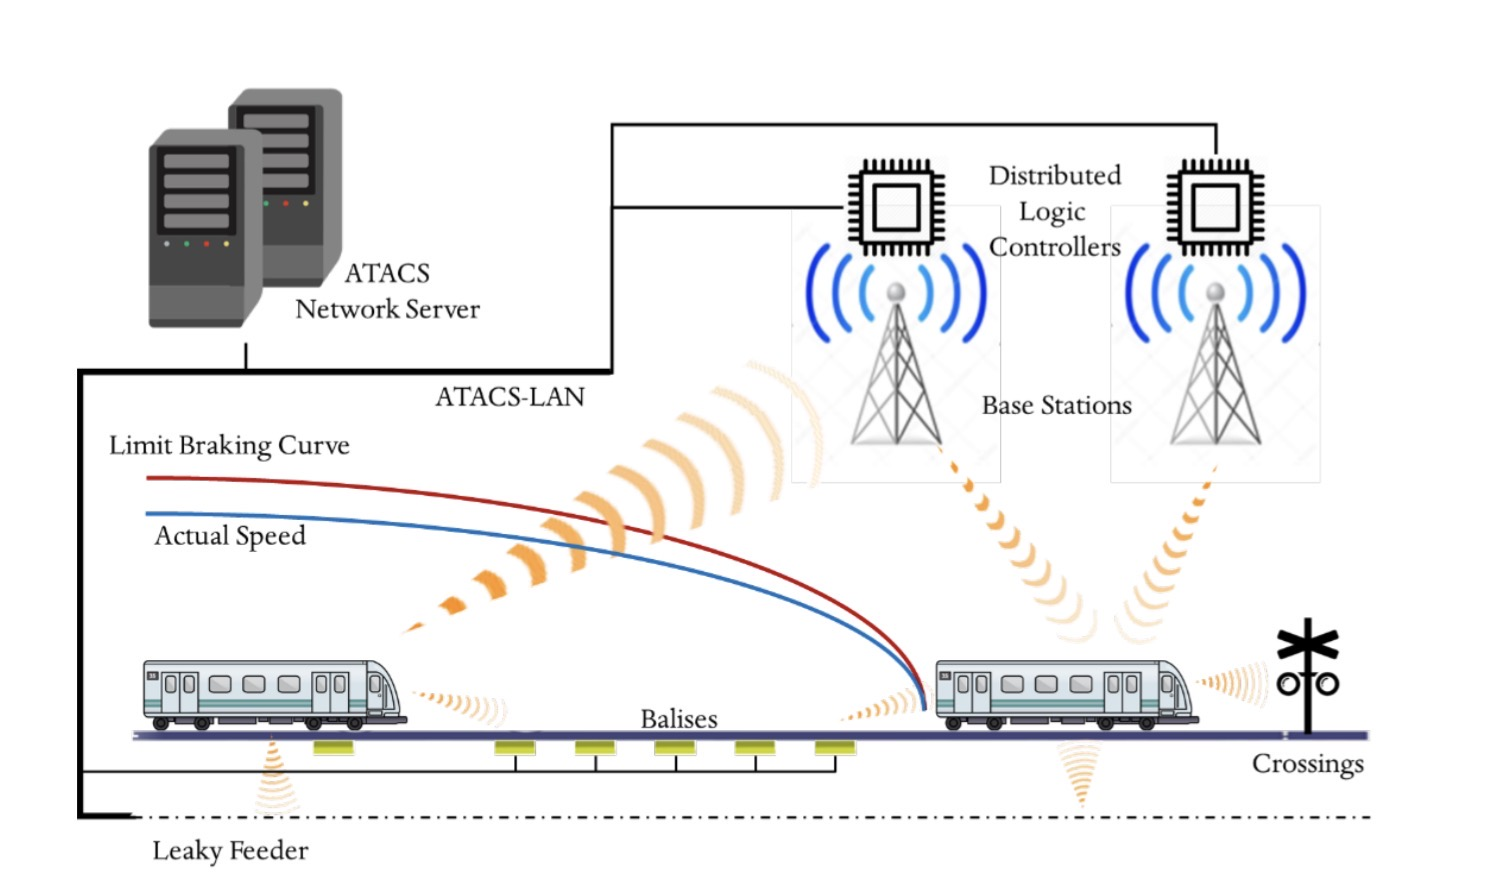
\includegraphics[width=0.8\textwidth]{res/Bahn_Infrastruktur.jpg}
\caption{Überblick über die Schieneninfrastruktur~\cite{xiangliuCyber2020}}
\label{fig:Schieneninfrastruktur}
\end{figure}

\begin{itemize}
    \item \textbf{Fahrzeugseitige Steuerungseinheit:} Eine \gls{obu}, ein \gls{evc} oder ein vergleichbarer Sicherheitsrechner verarbeitet Zugposition, Geschwindigkeit und Fahrterlaubnisse und überwacht daraus abgeleitete Bremskurven~\parencite[S. 10]{xiangliuCyber2020}~\parencite[S. 101--104]{trinckaufETCS2024}.
    \item \textbf{Streckenseitige Referenz- und Übertragungselemente:} Balisen oder andere \textit{Transponder} übertragen punktförmig Streckeninformationen und unterstützen die Positionsreferenzierung~\parencite[S. 10--11]{xiangliuCyber2020}~\parencite[S. 75--76]{trinckaufETCS2024}.
    \item \textbf{Kommunikationsschnittstelle:} Eine bidirektionale Funk- oder Kabelverbindung transportiert sicherheitsrelevante Informationen wie Positionsberichte und Fahrterlaubnisse. Je nach System kommen unter anderem \gls{gsm-r}, \gls{tdma}-Funk oder \textit{Leaky-Coaxial}-Kabel (\gls{lcx}) zum Einsatz~\parencite[S. 9--14]{xiangliuCyber2020}.
\end{itemize}

Diese gemeinsamen Komponenten bilden den Vergleichsrahmen; konkrete Schutzmechanismen wie Angriffserkennung, Segmentierung oder dynamische Netzwerkverfahren werden erst in der Diskussion hinsichtlich ihres Beitrags und ihrer Grenzen bewertet.

\subsection{\texorpdfstring{Europäische Eisenbahnarchitektur: \gls{ertms} und \gls{etcs}}{Europäische Eisenbahnarchitektur: ERTMS und ETCS}}
\label{sec:Europäische_Eisenbahnarchitektur_ERTMS_und_ETCS}

Für Europa werden vier Aspekte betrachtet: zunächst die funktionale Struktur der \gls{etcs}-\textit{Level}, anschließend die Migration von \gls{gsm-r} zu \gls{frmcs}, danach der Integritäts- und Authentizitätsschutz der Zug-Strecken-Kommunikation und schließlich Architekturen zur Trennung unterschiedlich schnell alternder \textit{Safety}- und \textit{Security}-Komponenten.

\subsubsection{Struktur und Funktionsweise}
\label{sec:Struktur_und_Funktionsweise}
Das \textit{European Rail Traffic Management System} (\gls{ertms}) definiert das \textit{European Train Control System} (\gls{etcs}) als einheitliches europäisches Zugsicherungssystem~\parencite[S. 49]{trinckaufETCS2024}. Die Interaktion zwischen Zug und Streckenausrüstung wird über \textit{Level} strukturiert:

% \begin{figure}[htbp!]
%     \centering
%     \begin{subfigure}[t]{0.48\linewidth}
%         \centering
%         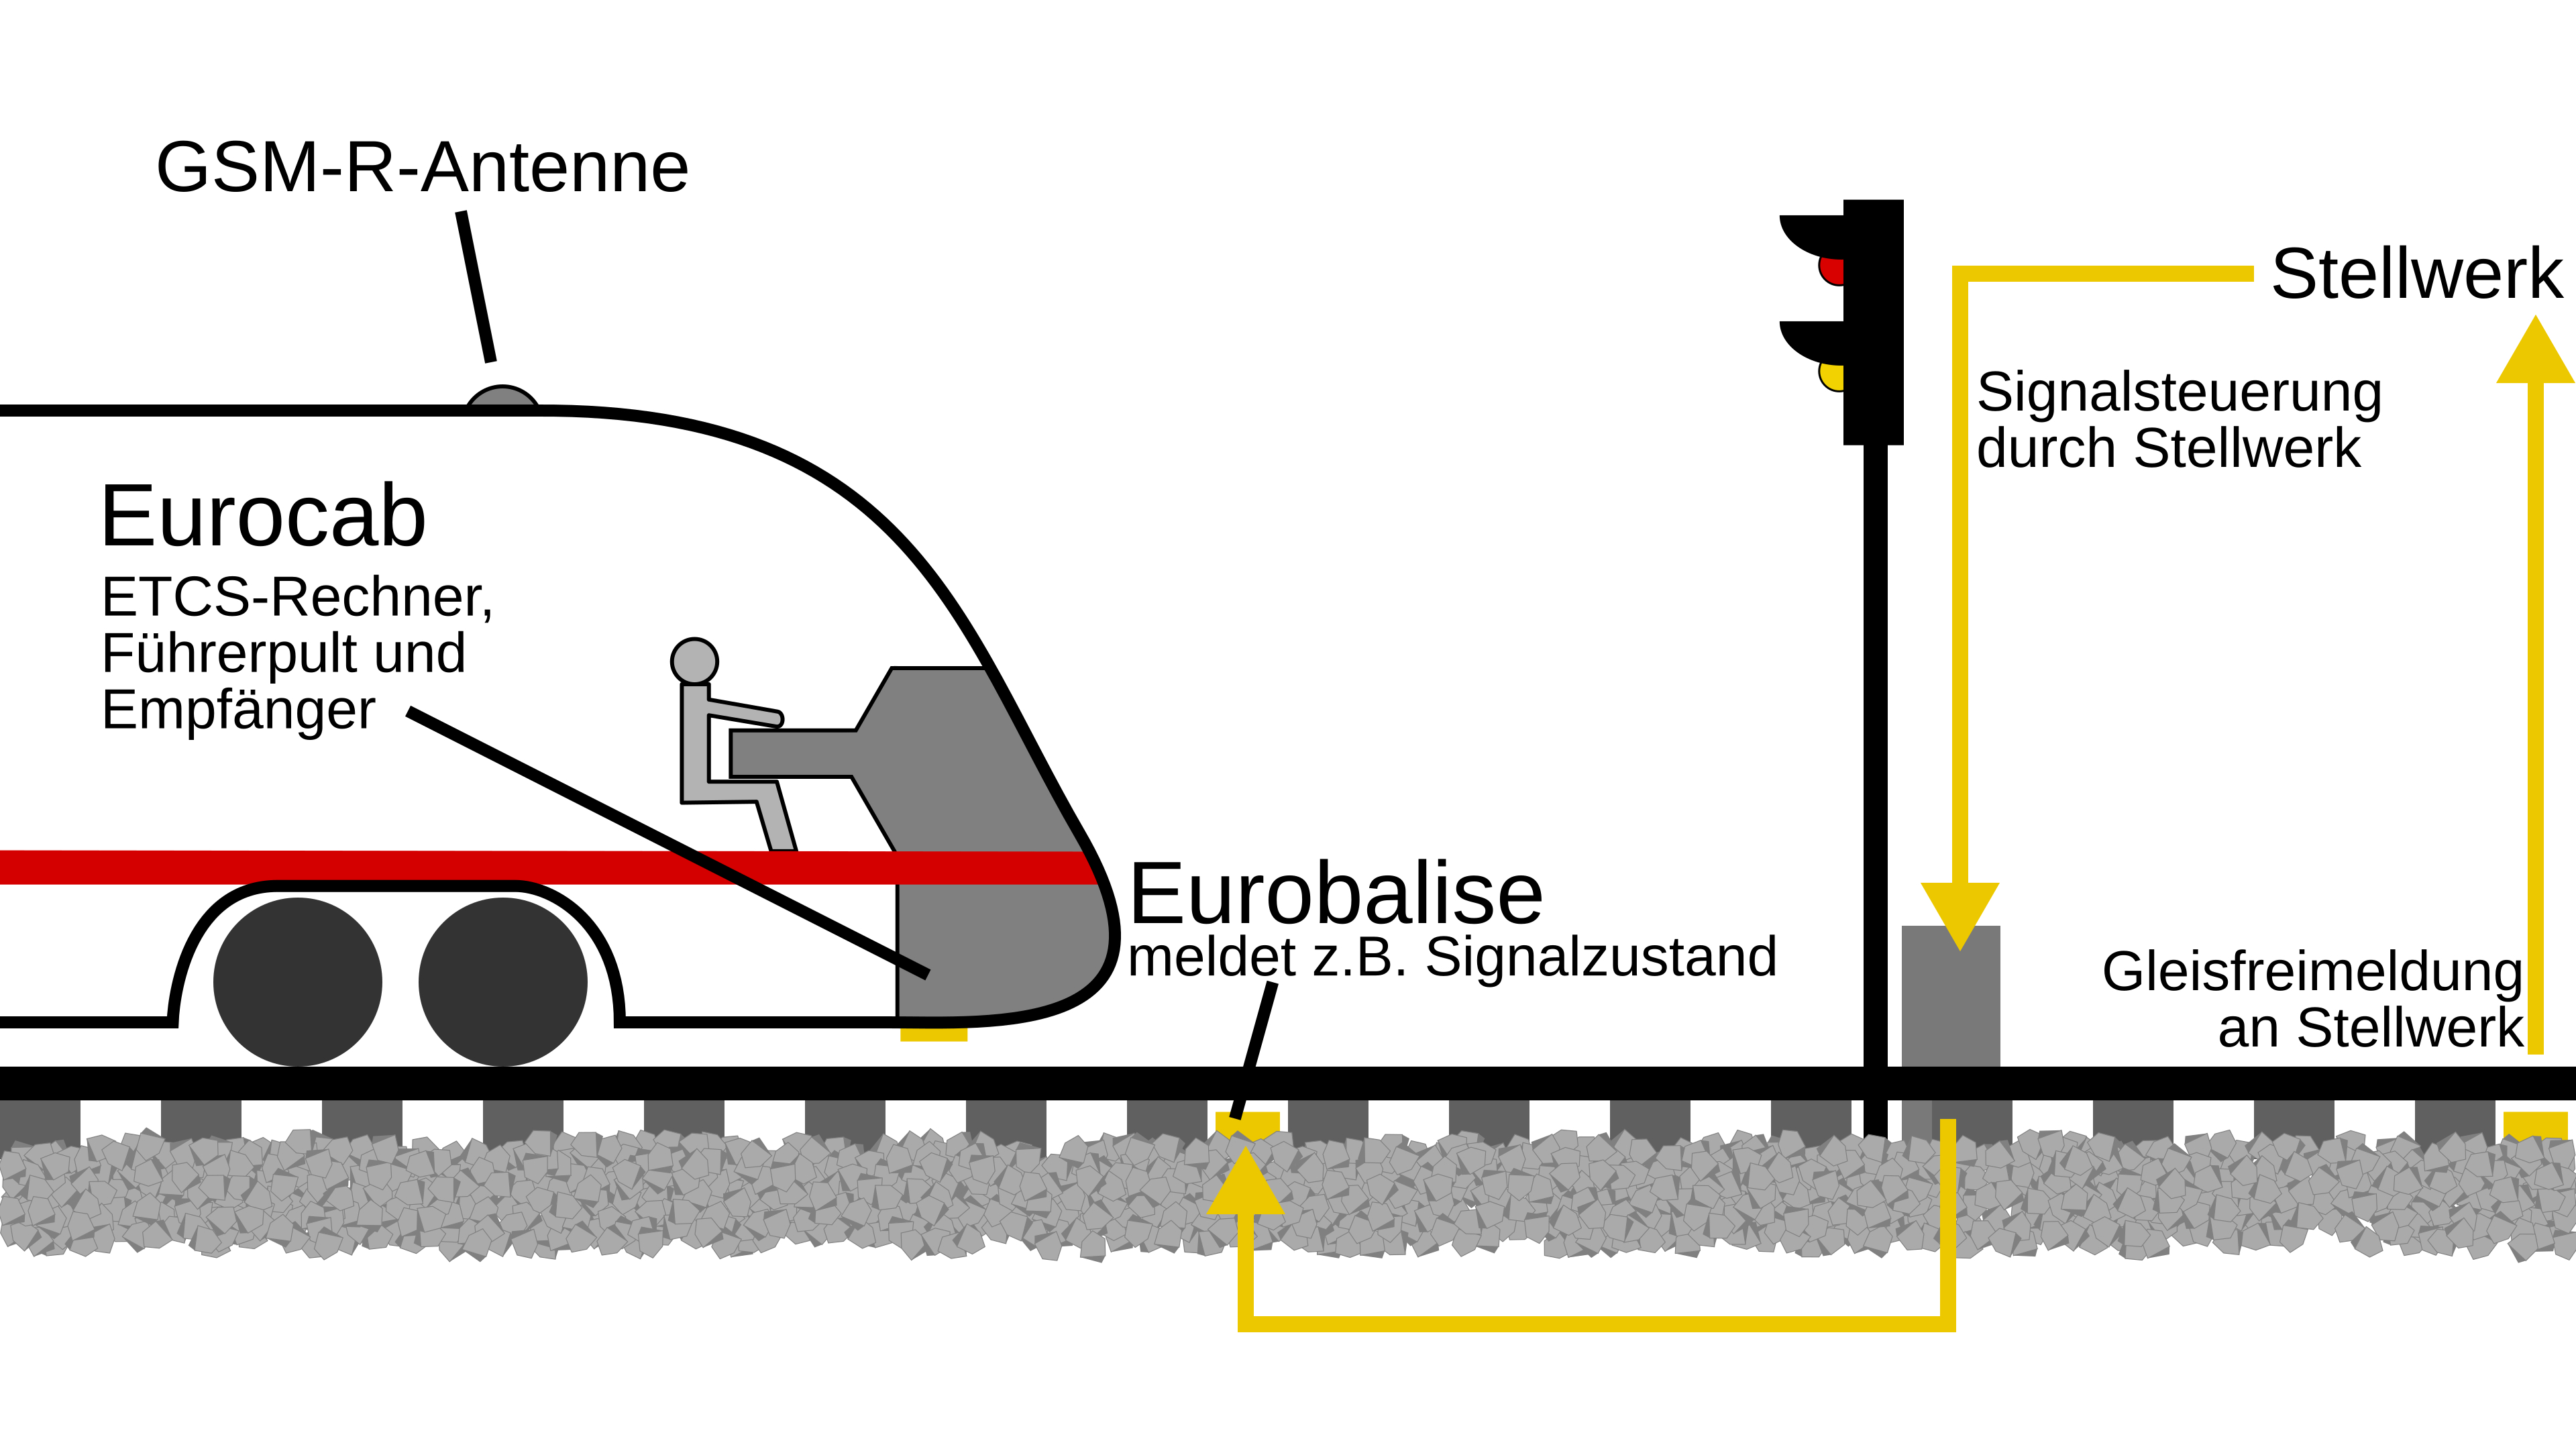
\includegraphics[width=\linewidth]{res/ECTS_Level1.jpg}
%         \caption{\gls{etcs} \textit{Level} 1~\cite{sansculotteETCSLevel1}}
%         \label{fig:ETCS-level-1}
%     \end{subfigure}%
%     \hfill
%     \begin{subfigure}[t]{0.48\linewidth}
%         \centering
%         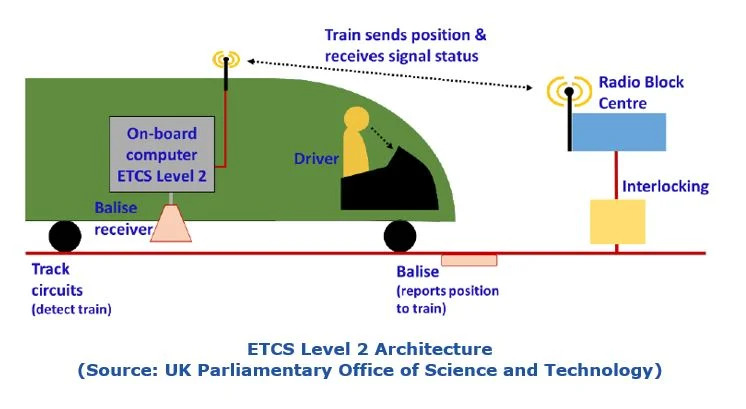
\includegraphics[width=\linewidth]{res/ECTS_Level2.jpg}
%         \caption{\gls{etcs} \textit{Level} 2~\cite{arcETCS}}
%         \label{fig:ETCS-level-2}
%     \end{subfigure}
%     \caption{ETCS Level 1 und Level 2}
%     \label{fig:ETCS-level-comparison}
% \end{figure}

\begin{itemize}
    
    \begin{figure}[H]
    \centering
    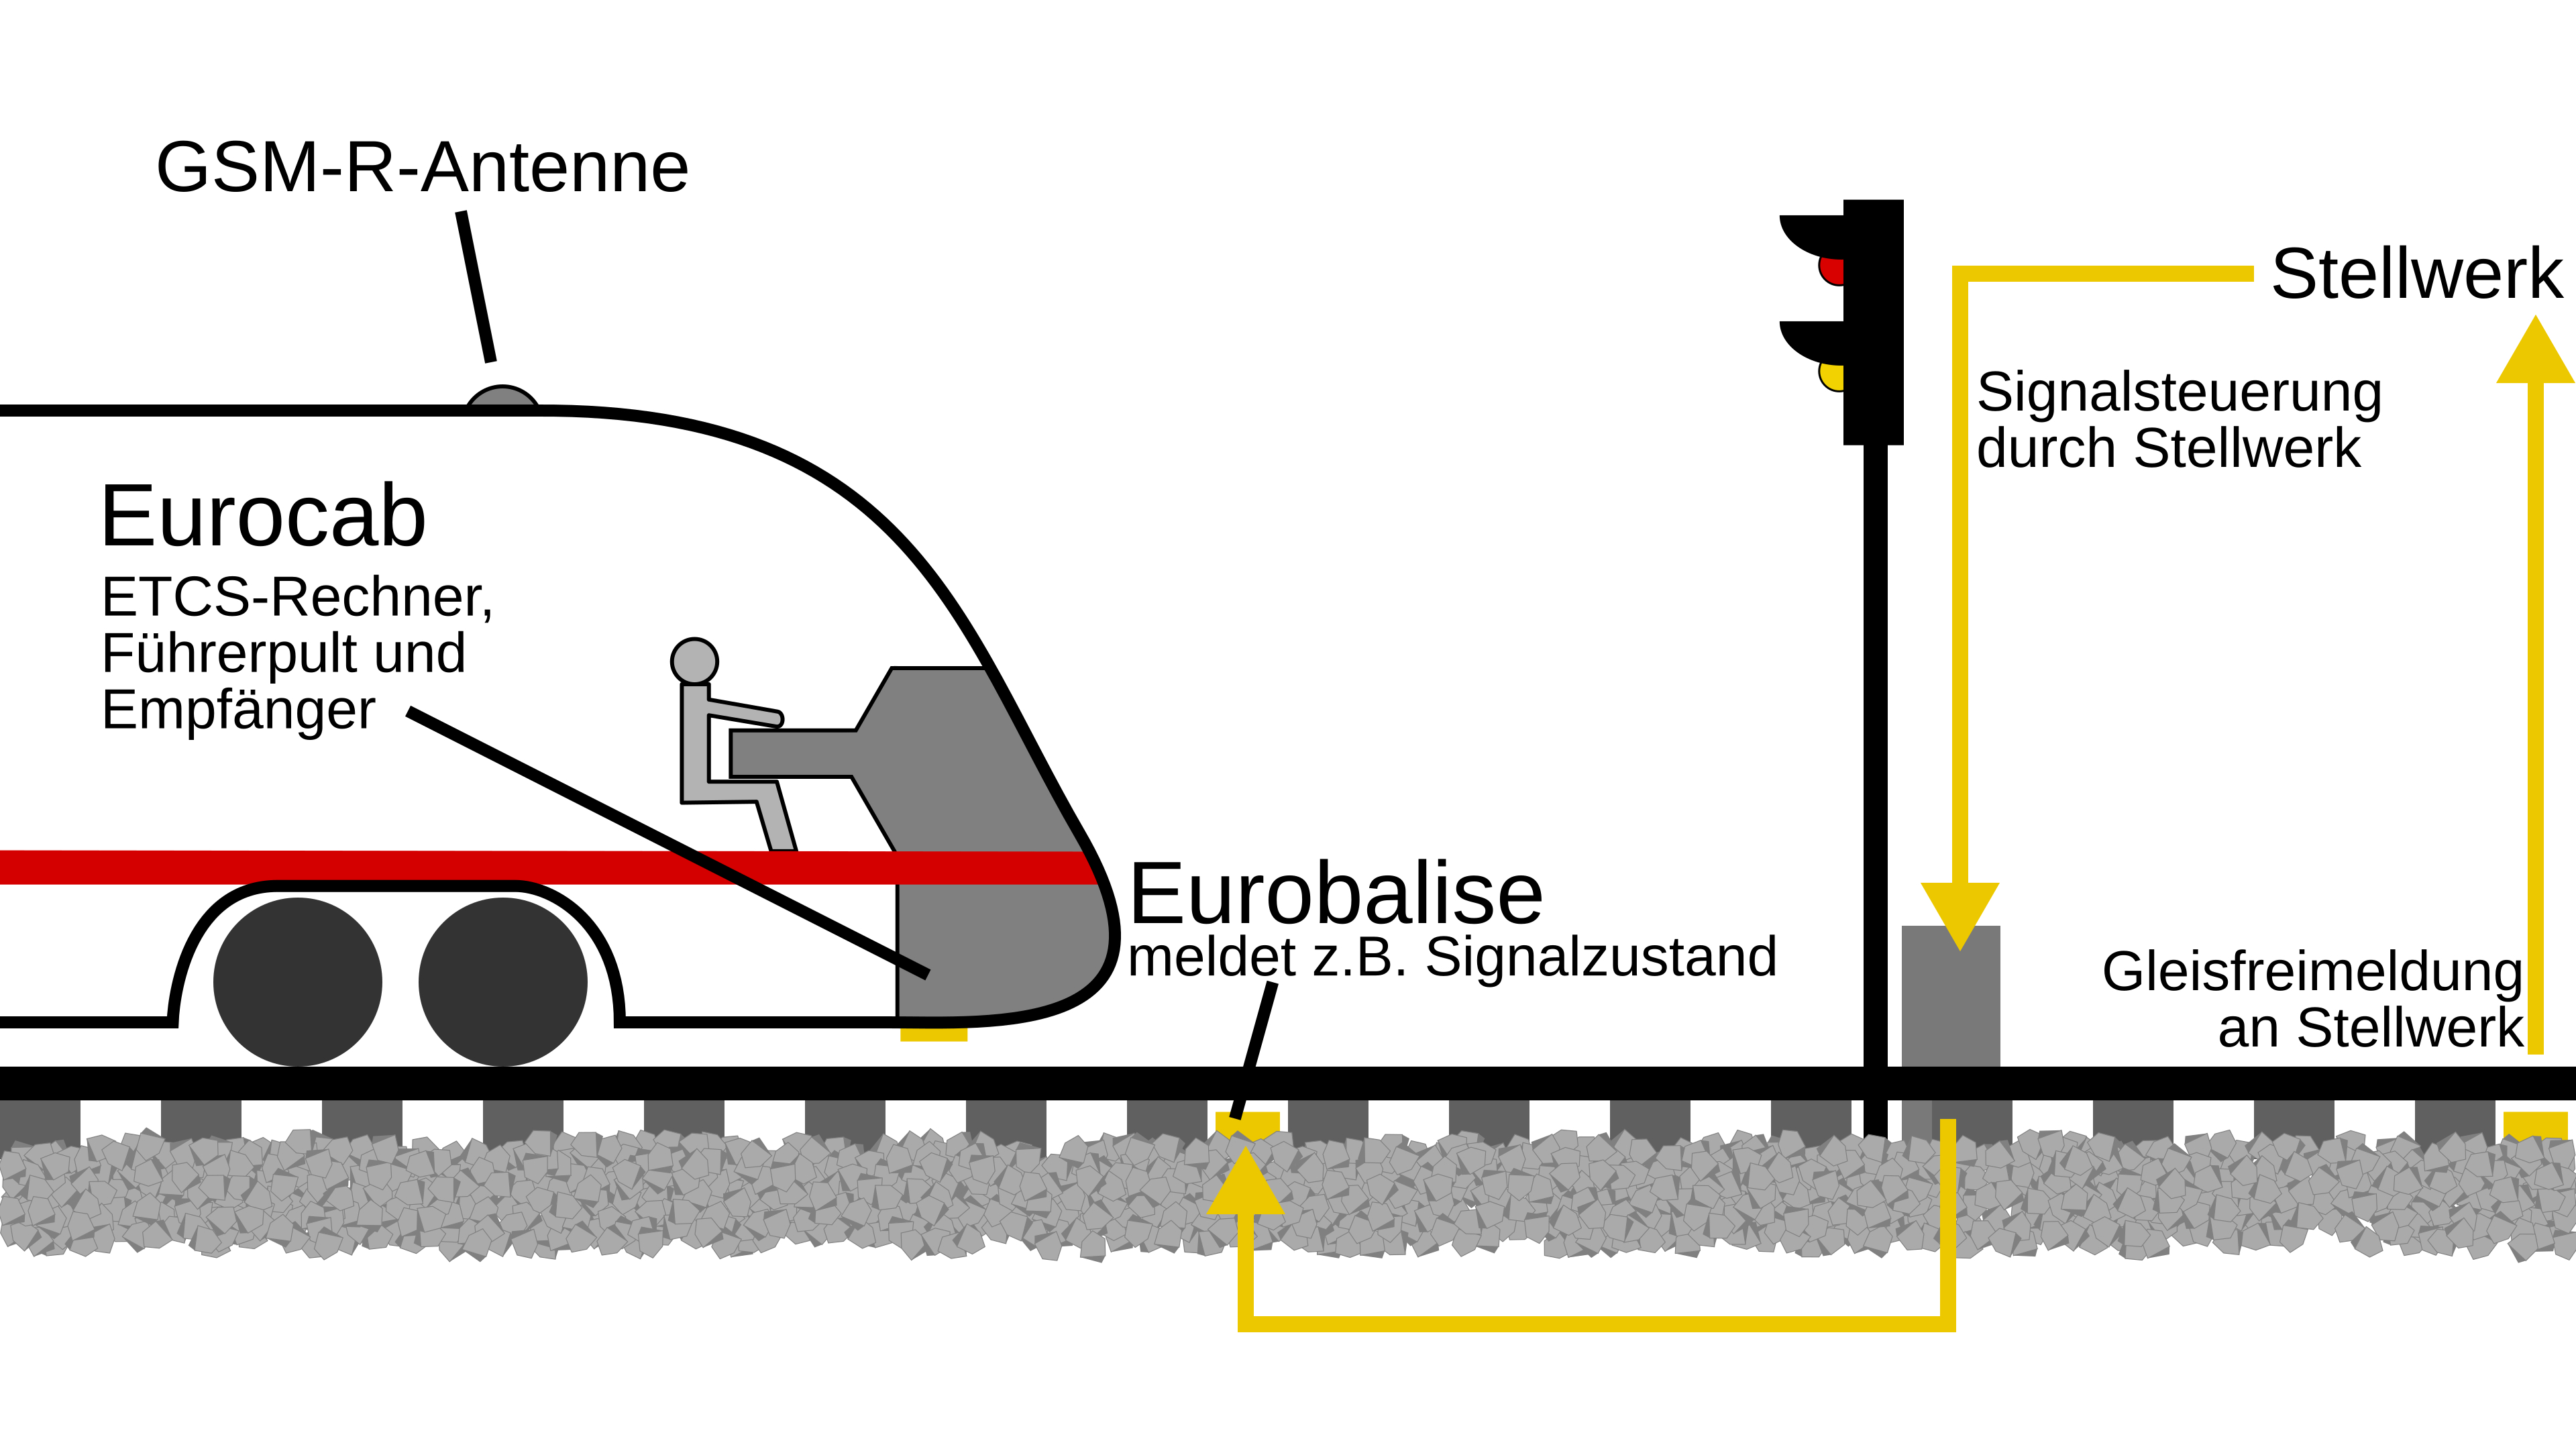
\includegraphics[width=0.7\textwidth]{res/ECTS_Level1.jpg}
    \caption{\gls{etcs} \textit{Level} 1~\cite{sansculotteETCSLevel1}}
    \label{fig:ETCS-level-1}
    \end{figure}
    
    \item \textbf{\gls{etcs} \textit{Level} 1:} Fahrterlaubnisse werden punktförmig über Eurobalisen an das Fahrzeug übertragen; die Streckeneinteilung beruht weiterhin auf festen Blockabschnitten~\parencite[S. 50, 71]{trinckaufETCS2024}.
    
    \begin{figure}[H]
    \centering
    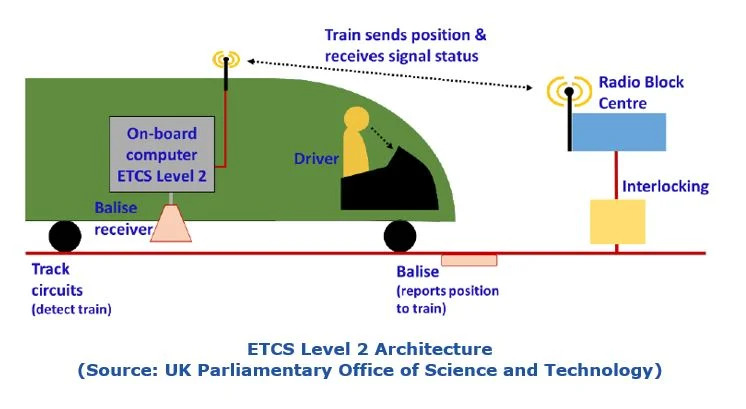
\includegraphics[width=0.65\textwidth]{res/ECTS_Level2.jpg}
    \caption{\gls{etcs} \textit{Level} 2~\cite{arcETCS}}
    \label{fig:ETCS-level-2}
    \end{figure}
    
    \item \textbf{\gls{etcs} \textit{Level} 2:} Zwischen Fahrzeug und \gls{rbc} besteht eine kontinuierliche Funkverbindung. Das \gls{rbc} verarbeitet Stellwerksinformationen und Positionsberichte und übermittelt daraus erzeugte \textit{Movement Authorities}; ortsfeste Signale sind technisch nicht mehr zwingend erforderlich~\parencite[S. 71, 89--90]{trinckaufETCS2024}.
    
    \begin{figure}[H]
    \centering
    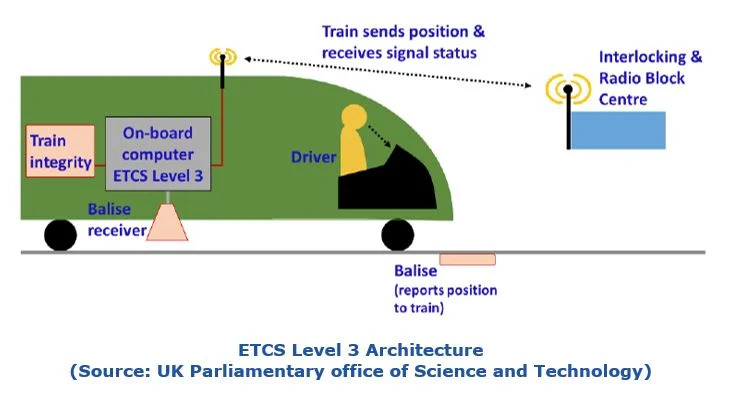
\includegraphics[width=0.65\textwidth]{res/ECTS_Level3.jpg}
    \caption{\gls{etcs} \textit{Level} 3~\cite{arcETCS}}
    \label{fig:ETCS-level-3}
    \end{figure}

    \item \textbf{\gls{etcs} \textit{Level} 3:} Die Zugvollständigkeit wird fahrzeugseitig überwacht, wodurch gleisseitige Freimeldung reduziert und ein \textit{Moving Block} ermöglicht werden kann~\parencite[S. 471--472]{trinckaufETCS2024}.
\end{itemize}

\subsubsection{\texorpdfstring{Nachfolgetechnologie \gls{rmr} und \gls{frmcs}}{Nachfolgetechnologie RMR und FRMCS}}
\label{sec:Nachfolgetechnologie_RMR_und_FRMCS}
Zur Ablösung der \gls{2g}-basierten \gls{gsm-r}-Infrastruktur wird im Rahmen von \textit{Railway Mobile Radio} (\gls{rmr}) das \textit{Future Railway Mobile Communication System} (\gls{frmcs}) entwickelt~\parencite[S. 49, 123]{trinckaufETCS2024}. Zentral ist die funktionale Trennung von Anwendung, bahnspezifischen Diensten und Übertragungsschicht. Diese \textit{Bearer Independence} soll es ermöglichen, Übertragungstechnologien weiterzuentwickeln, ohne die sicherheitskritische Anwendungslogik bei jedem Wechsel grundlegend neu zu gestalten~\parencite[S. 123, 211]{trinckaufETCS2024}. Fahrzeugseitig unterstützt die \textit{Telecom On-Board Architecture} (\gls{toba}) diese Modularisierung über standardisierte Schnittstellen~\parencite[S. 123, 219]{trinckaufETCS2024}.

\subsubsection{\texorpdfstring{Kryptographische Schutzmechanismen und Schlüsselmanagement in \gls{etcs}}{Kryptographische Schutzmechanismen und Schlüsselmanagement in ETCS}}
\label{sec:Kryptographische_Schutzmechanismen_und_Schlüsselmanagement_in_ETCS}
Bei funkbasierten \gls{etcs}-Verbindungen schützt \textit{EuroRadio} insbesondere Authentizität und Integrität der zwischen Fahrzeug und \gls{rbc} übertragenen Anwendungsdaten, während \gls{gsm-r} die Übertragungsinfrastruktur bereitstellt~\parencite[S. 744, 751]{chothiaAttack2017}. Der traditionelle \textit{EuroRadio}-Schutz nutzt einen \gls{mac} auf Basis von \gls{iso} 9797-1 mit \gls{des}/\gls{3des}; die symmetrischen Schlüssel werden über ein hierarchisches \textit{Key Management System} verwaltet~\parencite[S. 751]{chothiaAttack2017}~\parencite[S. 90, 100]{trinckaufETCS2024}. Neuere Spezifikationen richten die Kommunikation stärker auf \gls{ip}-basierte Sicherheitsmechanismen mit \gls{tls} und zertifikatsbasierter \gls{pki} aus~\parencite[S. 105, 211]{trinckaufETCS2024}.

\subsubsection{\texorpdfstring{Sichere \textit{Software}-Partitionierung: \gls{mils} und \textit{Separation Kernels}}{Sichere Software-Partitionierung: MILS und Separation Kernels}}
\label{sec:Sichere_Software-Partitionierung_MILS_und_Separation_Kernels}
Da \textit{Safety}-Anwendungen und \textit{Security}-Komponenten unterschiedliche Lebenszyklen besitzen, werden in High-Assurance-Architekturen Partitionierungsansätze wie \gls{mils} untersucht. Ein zertifizierter \textit{Separation Kernel} trennt sicherheitskritische Steuerungslogik von Kommunikations- und Sicherheitsdiensten, sodass Änderungen an einer Partition nicht zwangsläufig den gesamten Sicherheitsnachweis betreffen~\parencite[S. 31--35]{schulzIntegration2019}~\parencite[S. 80--83]{tverdyshevCertMILS2019}. Für ortsfeste Leit- und Sicherungstechnik ergänzt \gls{iec} 62443 diesen Ansatz durch \textit{Zones} und \textit{Conduits}, die Kommunikationsbeziehungen segmentieren und kontrollieren~\parencite[S. 33]{schulzIntegration2019}~\parencite[S. 43]{h.tsukisawaStandardization2024}.

\subsection{Japanische Eisenbahnarchitektur}
\label{sec:Japanische_Eisenbahnarchitektur}

Die japanische Seite wird entlang ihrer institutionellen Heterogenität, der Entwicklung von \gls{atc} zu funkbasierten Systemen, dem aktuellen \gls{rtri}-Ansatz zur vom Übertragungsweg unabhängigen Zugsteuerung und der dort eingesetzten kryptographischen Absicherung betrachtet. Im Unterschied zum europäischen Standardisierungsrahmen ist dabei zwischen Betreiberpraxis und veröffentlichten Forschungsansätzen zu unterscheiden.

\subsubsection{Historische Entwicklung und betreiberspezifische Heterogenität}
\label{sec:Historische_Entwicklung_und_betreiberspezifische_Heterogenität}
Die Privatisierung der \textit{Japan National Railways} (\gls{jnr}) im Jahr 1987 führte zu mehreren regionalen \gls{jr}-Gesellschaften und weiteren privaten Bahnbetreibern~\parencite[S. 47]{yanaseJapanese2011}. Nationale Vorgaben definieren Mindest- und Funktionsanforderungen, während Betreiber eigene technische Implementierungsstandards festlegen können~\parencite[S. 48--49, 51]{yanaseJapanese2011}. Dadurch entstand eine stärker betreiber- und streckenspezifische Systemlandschaft als im europäischen \gls{ertms}-Rahmen.

\subsubsection{\texorpdfstring{\gls{atc} und \gls{atacs}}{ATC und ATACS}}
\label{sec:ATC_und_ATACS}
\textit{Digital} \gls{atc} (\gls{d-atc}) überträgt digitale Informationen über codierte Schienenstromkreise, während die fahrzeugseitige Einheit daraus Bremskurven berechnet~\parencite[S. 44--45]{h.tsukisawaStandardization2024}. \gls{atacs} ist demgegenüber ein von \gls{jr} \textit{East} entwickeltes funkbasiertes Zugsteuerungssystem. Das Fahrzeug bestimmt seine Position unter anderem mit Radsensoren und Transpondern und übermittelt sie über \gls{tdma}-Funk beziehungsweise \gls{lcx}; auf dieser Grundlage werden dynamische Fahr- und Bremsinformationen erzeugt~\parencite[S. 13--14]{xiangliuCyber2020}~\parencite[S. 6, 8]{iwamotoTrain2024}.

\subsubsection{\texorpdfstring{Unabhängige Zugsteuerung und \gls{iec} 62280}{Unabhängige Zugsteuerung und IEC 62280}}
\label{sec:Unabhängige_Zugsteuerung_und_IEC_62280}
Aktuelle Arbeiten des \textit{Railway Technical Research Institute} (\gls{rtri}) untersuchen ein \textit{Train Control System Independent of Communication Transmission Paths}~\parencite[S. 1--3]{iwamotoTrain2024}. Das Konzept trennt Sicherheitssteuerung und Informationsübertragung und behandelt den Übertragungsweg entsprechend den Bedrohungskategorien der \gls{iec} 62280 als potenziell unzuverlässig~\parencite[S. 1, 4, 7]{iwamotoTrain2024}. Fahrterlaubnisse werden nur bei positiv bestätigten Daten erteilt; für Notstopps wird dagegen das Ausbleiben zyklischer Nachrichten als Gefahr interpretiert~\parencite[S. 10--12]{iwamotoTrain2024}. Dadurch können prinzipiell auch öffentliche Netze wie \gls{5g} oder \gls{wi-fi} als Transportmedium einbezogen werden, sofern die sicherheitsrelevante Logik ihre Annahmen unabhängig davon durchsetzt~\parencite[S. 3, 10]{iwamotoTrain2024}.

\subsubsection{Kryptographische Absicherung in Japan}
\label{sec:Kryptographische_Absicherung_in_Japan}
Im untersuchten \gls{rtri}-Ansatz wird zur Authentisierung und Fälschungserkennung ein \textit{Hash-based Message Authentication Code} auf Basis von \gls{sha-256} (\gls{hmac-sha256}) eingesetzt~\parencite[S. 12]{iwamotoTrain2024}. Konkrete Details zur Schlüsselverwaltung und zu operativen Sicherheitskonfigurationen einzelner japanischer Betreiber sind in öffentlich zugänglichen Quellen jedoch nur eingeschränkt dokumentiert. Diese Evidenzlücke muss beim späteren Vergleich ausdrücklich berücksichtigt werden.

\section{Methodik}
\label{sec:Methodik}

Dieses Kapitel beschreibt, wie aus der heterogenen Literatur eine nachvollziehbare Vergleichsbasis abgeleitet wird. Zunächst wird das Forschungsdesign erläutert, anschließend werden Auswahl und Gewichtung der Quellen begründet. Danach werden Untersuchungsumfang und Einschränkungen abgegrenzt. Abschließend wird dargestellt, anhand welcher Kriterien die europäischen und japanischen Ansätze in der Diskussion bewertet werden.

\subsection{Forschungsdesign: Strukturierte Literaturanalyse}
\label{sec:Forschungsdesign_Strukturierte_Literaturanalyse}

Die Arbeit folgt einer strukturierten, vergleichenden Literaturanalyse. Untersucht werden technische Standards, offizielle Dokumentationen, wissenschaftliche Veröffentlichungen und ausgewählte Betreiber- beziehungsweise Branchenquellen zur sicherheitskritischen Zug-Strecken-Kommunikation. Ziel ist nicht die vollständige Beschreibung einzelner Systeme, sondern die Ableitung und Gegenüberstellung von Sicherheitsprinzipien, Abhängigkeiten und Grenzen. Direkte Penetrationstests oder experimentelle Manipulationen realer Eisenbahninfrastruktur sind wegen der sicherheitskritischen und betrieblichen Auswirkungen nicht Bestandteil der Untersuchung.

\subsection{Quellenauswahl und Evidenzgewichtung}
\label{sec:Quellenauswahl_und_Evidenzgewichtung}

Die Quellen werden nach ihrer Funktion im Argument unterschiedlich gewichtet. Technische Standards und offizielle Systemdokumentationen dienen primär zur Beschreibung spezifizierter Architekturen und Schnittstellen. Wissenschaftliche Sicherheitsanalysen werden herangezogen, wenn konkrete Schwachstellen, Angriffsmöglichkeiten oder Schutzmechanismen bewertet werden. Veröffentlichte Störungsberichte und Betreiberinformationen dienen ergänzend dazu, theoretische Annahmen mit beobachtbaren Betriebsereignissen zu kontrastieren. Wo eine Aussage nur durch einen Forschungsprototyp oder eine einzelne Implementierung belegt ist, wird sie nicht ohne Weiteres auf eine gesamte Region übertragen. Diese Unterscheidung ist insbesondere für Japan relevant, weil öffentlich verfügbare Details einzelner Betreiber deutlich begrenzter sind als die Dokumentation des europäischen \gls{ertms}-Rahmens.

\subsection{Vergleichsrahmen und Einschränkungen}
\label{sec:Vergleichsrahmen_und_Einschränkungen}

Der Vergleich konzentriert sich auf Kommunikationsbeziehungen zwischen Fahrzeugen und streckenseitigen beziehungsweise zentralen Steuerungskomponenten. Betrachtet werden sicherheitsrelevante Informationen wie \textit{Movement Authorities}, Positionsmeldungen, Geschwindigkeitsinformationen und Notstopp-Nachrichten. Für Europa stehen \gls{ertms}, \gls{etcs}, \gls{gsm-r}, \textit{EuroRadio} und die Migration zu \gls{frmcs} im Mittelpunkt. Für Japan werden \gls{d-atc}, \gls{atacs} sowie der veröffentlichte \gls{rtri}-Ansatz zur vom Übertragungsweg unabhängigen Zugsteuerung betrachtet.

Die Analyse beruht ausschließlich auf öffentlich zugänglicher Literatur und ist daher kein empirischer Sicherheitstest konkreter Netze. Nicht betrachtet werden Fahrgast-\gls{wlan}, Fahrgastinformation, \textit{Ticketing} oder allgemeine Unternehmens-\gls{it}. Außerdem ist die Vergleichbarkeit dadurch begrenzt, dass auf europäischer Seite produktive Bestands- und Migrationssysteme, auf japanischer Seite teilweise betreiberspezifische Systeme und teilweise Forschungsansätze gegenübergestellt werden. Ergebnisse werden deshalb als architektonische Tendenzen und nicht als flächendeckende Aussagen über alle europäischen oder japanischen Bahnen interpretiert.

\subsection{Bewertungsverfahren}
\label{sec:Bewertungsverfahren}

Aus Forschungsfrage und theoretischem Rahmen werden fünf Vergleichskriterien abgeleitet:

\begin{enumerate}
    \item \textbf{Standardisierung und Interoperabilität:} Wie stark sind Schnittstellen und Kommunikationsmechanismen vereinheitlicht, und welche Auswirkungen hat dies auf Migration und gemeinsame Abhängigkeiten?
    \item \textbf{Integrität und Authentizität:} Mit welchen Mechanismen werden Manipulation, Fälschung und Wiederholung sicherheitskritischer Nachrichten adressiert?
    \item \textbf{Verfügbarkeit und Resilienz:} Wie reagiert das System auf Kommunikationsverlust, \textit{Jamming}, Ausfälle oder Fehler gemeinsamer Infrastruktur?
    \item \textbf{Architektonische Entkopplung und Aktualisierbarkeit:} In welchem Umfang können Übertragungstechnik und \textit{Security}-Mechanismen verändert werden, ohne die \textit{Safety}-Logik vollständig neu zu qualifizieren?
    \item \textbf{Evidenz und Reifegrad:} Beruht die Bewertung auf produktiv eingesetzten Systemen, verbindlichen Standards oder Forschungsprototypen, und welche Aussagen sind deshalb belastbar?
\end{enumerate}

Die Literatur wird zunächst diesen Kriterien zugeordnet. Anschließend werden Gemeinsamkeiten und Unterschiede qualitativ verglichen und auf verbleibende Sicherheitsgrenzen untersucht. Auf eine numerische Bewertung wird verzichtet, weil Reifegrad, Dokumentationstiefe und betrachtete Systemgenerationen zwischen den Quellen zu unterschiedlich sind, um eine scheinbar präzise Punktzahl methodisch zu rechtfertigen.

\section{Diskussion}
\label{sec:Diskussion}

Dieses Kapitel wendet die in Kapitel~\ref{sec:Methodik} definierten Kriterien auf die zuvor beschriebenen Systeme an. Zunächst werden die zentralen verwandten Arbeiten eingeordnet und ihre Rolle für die vorliegende Untersuchung abgegrenzt. Danach folgt die eigentliche vergleichende Bewertung von Standardisierung, Nachrichtenschutz, Verfügbarkeit und Aktualisierbarkeit. Abschließend werden aus dem Vergleich konkrete Architekturprinzipien und Forschungslücken abgeleitet. Der Schwerpunkt liegt damit nicht auf einer erneuten technischen Beschreibung, sondern auf der Interpretation der Befunde im Hinblick auf die Forschungsfrage.

\subsection{Stand der Forschung und verwandte Arbeiten}
\label{sec:Stand_der_Forschung_und_verwandte_Arbeiten}
Die vorliegende Arbeit verbindet Forschungsstränge, die in der Literatur überwiegend getrennt behandelt werden: kryptographische Protokollanalysen, generische Modelle funkbasierter Zugsteuerung, High-Assurance-Architekturen sowie Standardisierung und Migrationskonzepte. Der eigene Beitrag besteht nicht in einem neuen Protokoll, sondern in der vergleichenden Einordnung dieser Befunde für Europa und Japan.

\subsubsection{Kryptographische Protokollanalysen und Kommunikationsschwachstellen}
Chothia et al. zeigen, dass der traditionelle \textit{EuroRadio}-Integritätsschutz aufgrund seiner \gls{des}-basierten Konstruktion kryptographische Schwächen besitzt und unter bestimmten Voraussetzungen gefälschte Nachrichten ermöglicht~\parencite[S. 743--756]{chothiaAttack2017}. Gaggero et al. erweitern die Perspektive auf drahtlose Schwachstellen von \gls{ertms} und betonen insbesondere das Verfügbarkeitsproblem: Ein Kommunikationsverlust führt aus \textit{Safety}-Gründen zu einem restriktiven Zustand und kann dadurch für \textit{Denial-of-Service}-Angriffe ausgenutzt werden~\parencite[S. 52--61]{gaggeroSurvey2024}. Diese Arbeiten liefern damit die Grundlage für die Bewertung von Integrität und Verfügbarkeit, vergleichen jedoch keine europäischen und japanischen Migrationsansätze.

\subsubsection{Funkbasierte Zugsteuerungsarchitekturen und Systemmodelle}
Liu et al. stellen ein herstellerneutrales Komponenten- und Risikomodell für vernetzte Zugsteuerungssysteme bereit, das in dieser Arbeit als gemeinsamer technischer Bezugsrahmen dient~\parencite[S. 1--15]{xiangliuCyber2020}. Iwamoto et al. beschreiben dagegen mit der vom Übertragungsweg unabhängigen Zugsteuerung einen spezifischen japanischen Forschungsansatz, der die Sicherheitslogik vom Transportmedium entkoppelt~\parencite[S. 1--12]{iwamotoTrain2024}. Tsukisawa et al. ergänzen diese Sicht um Standardisierung und Segmentierung nach \gls{iec} 62443~\parencite[S. 41--43]{h.tsukisawaStandardization2024}. Für die vorliegende Arbeit sind diese Quellen besonders relevant, weil sie die funktionale Entkopplung als regionsübergreifendes Vergleichsmerkmal sichtbar machen.

\subsubsection{High-Assurance-Architekturen, Angriffserkennung und dynamische Abwehr}
Schulz et al. und Tverdyshev untersuchen \gls{mils} und \textit{Separation Kernels} zur Isolation unterschiedlich kritischer Softwarekomponenten und zur Entkopplung von Lebenszyklen~\parencite[S. 31--35]{schulzIntegration2019}~\parencite[S. 80--83]{tverdyshevCertMILS2019}. Melaragno et al. adressieren mit \gls{rrids} die passive Angriffserkennung im Bahnfunk, während Poschinger et al. die Einsatzgrenzen von \gls{mtd}-Verfahren in zeitkritischen Netzen untersuchen~\parencite[S. 39--48]{melaragnoRail2016}~\parencite[S. 66--68, 121]{poschingerOpenMTD2020}. Diese Arbeiten werden hier nicht als eigenständige Zielarchitekturen, sondern als ergänzende Mechanismen bewertet.

\subsubsection{Umfassende Systemliteratur}
Trinckauf et al. liefern mit \textit{ETCS in Deutschland} die technische Gesamtgrundlage für \gls{etcs}, \gls{rmr}/\gls{frmcs}, Baselines und das Zusammenspiel von \textit{Safety} und \textit{Security}~\parencite[S. 49, 123, 204--211]{trinckaufETCS2024}. Im Unterschied dazu fokussiert die vorliegende Arbeit nicht auf die vollständige Beschreibung eines nationalen \gls{etcs}-Rollouts, sondern auf die sicherheitsbezogene Vergleichbarkeit mit japanischen Ansätzen.

\subsection{Sicherheitsarchitektur: Interoperabilität \textit{vs.} betreiberspezifische Diversität}
\label{sec:Sicherheitsarchitektur_Interoperabilität_vs_Betreiberspezifische_Diversität}
Europas zentrale Stärke ist der gemeinsame interoperable Rahmen von \gls{ertms}/\gls{etcs}~\parencite[S. 49]{trinckaufETCS2024}. Einheitliche Schnittstellen vereinfachen grenzüberschreitenden Betrieb, gemeinsame Zertifizierung und langfristig auch koordinierte Migrationen. Dieselbe Vereinheitlichung erzeugt jedoch eine gemeinsame Abhängigkeit: Wenn ein weit verbreitetes Protokoll oder eine gemeinsame Netzkomponente eine Schwachstelle besitzt, kann diese einen großen Teil der interoperablen Systemlandschaft betreffen. Die Herausforderung besteht daher nicht in der Standardisierung selbst, sondern darin, Standards so zu gestalten, dass kryptographische und kommunikative Komponenten ohne jahrzehntelange Bindung an veraltete Verfahren austauschbar bleiben.

Die japanische Heterogenität ist dagegen nicht automatisch als \textit{Security through Diversity} zu bewerten. Unterschiedliche Betreiber- und Herstellerlösungen können zwar die Reichweite eines einzelnen implementierungsspezifischen Fehlers begrenzen; daraus folgt jedoch kein inhärenter Sicherheitsvorteil. Heterogenität erschwert zugleich einheitliche Sicherheitsbewertungen, Patch-Prozesse, Personalqualifikation und interoperable Migrationen~\parencite[S. 47--49]{yanaseJapanese2011}. Die belastbarere Schlussfolgerung lautet deshalb: Diversität kann gemeinsame Fehlerdomänen verkleinern, erhöht aber die organisatorische und technische Sicherheitskomplexität.

Damit ergibt sich ein Zielkonflikt. Europa muss verhindern, dass Interoperabilität zu starrer technischer Homogenität wird; Japan muss verhindern, dass technische Autonomie zu fragmentiertem Sicherheitsmanagement führt. Beide Probleme sprechen für klar definierte Schnittstellen bei gleichzeitig austauschbaren Sicherheits- und Kommunikationskomponenten.

\subsection{Kryptographische Alterung und architektonische Entkopplung}
\label{sec:Kryptographische_Schwachstellen_und_MILS-basierte_Architekturkapselung}
Die von Chothia et al. nachgewiesenen Schwachstellen des traditionellen \textit{EuroRadio}-Schutzes zeigen ein grundsätzliches Lebenszyklusproblem: Ein Zugsicherungssystem kann über Jahrzehnte betrieben werden, während kryptographische Verfahren wesentlich schneller altern~\parencite[S. 751--754]{chothiaAttack2017}. Ein Austausch des Algorithmus allein löst dieses Problem nur temporär. Langfristig ist entscheidend, ob die Architektur spätere Sicherheitsupdates erlaubt, ohne den gesamten \textit{Safety}-Kern neu entwickeln oder vollständig neu qualifizieren zu müssen.

Hier ergänzen sich zwei in der Literatur getrennt behandelte Ideen. \gls{mils} und \textit{Separation Kernels} isolieren Kommunikations- und Sicherheitsdienste von der sicherheitskritischen Steuerungslogik~\parencite[S. 31--35]{schulzIntegration2019}. \gls{frmcs} verfolgt auf Netzebene ebenfalls eine funktionale Entkopplung von Anwendung, Dienst und Transport~\parencite[S. 123, 211]{trinckaufETCS2024}. Der japanische \gls{rtri}-Ansatz geht aus einer anderen Ausgangslage in dieselbe Richtung: Sicherheitsentscheidungen sollen nicht davon abhängen, dass ein bestimmter Übertragungsweg selbst vertrauenswürdig ist~\parencite[S. 1--4]{iwamotoTrain2024}.

Die gemeinsame Lehre ist daher nicht, dass eine bestimmte Technologie übernommen werden sollte, sondern dass \textit{Security}-Mechanismen als austauschbare, klar abgegrenzte Dienste behandelt werden müssen. Gleichzeitig darf diese Entkopplung nicht mit vollständiger Unabhängigkeit verwechselt werden: Gemeinsame Gateways, Identitätsdienste, Schlüsselverwaltung oder Zertifikatsinfrastrukturen können weiterhin zentrale Fehler- und Angriffspunkte bilden. Gerade diese verbleibenden gemeinsamen Abhängigkeiten sollten in Sicherheitsnachweisen explizit modelliert werden.

\subsection{Verfügbarkeit, Angriffserkennung und Redundanz}
\label{sec:IDS_MTD_und_Redundanzkonzepte}
Integritäts- und Authentizitätsschutz verhindern keine Funkstörung. Für Level~2/3 und vergleichbare funkbasierte Systeme bleibt Verfügbarkeit deshalb eine eigenständige Sicherheitsgrenze. Das \textit{Fail-Safe}-Prinzip sorgt dafür, dass Kommunikationsverlust nicht unkontrolliert in eine unsichere Fahrt übergeht; derselbe Mechanismus macht Verfügbarkeitsangriffe jedoch betrieblich wirksam~\parencite[S. 56--59]{gaggeroSurvey2024}. Der GSM-R-Vorfall vom 23. Juni 2026 zeigt zudem, dass nicht nur Angriffe, sondern auch Software-, Umschalt- und Betriebsfehler gemeinsame Kommunikationsinfrastruktur großflächig beeinträchtigen können~\cite{dbinfragoUrsacheZugfunkStoerung2026}.

Ergänzende Mechanismen adressieren unterschiedliche Teile dieses Problems. Passive \gls{ids} wie \gls{rrids} können anomale Nachrichtenfolgen erkennen, ohne selbst in den Steuerungspfad einzugreifen~\parencite[S. 60--63]{melaragnoRail2016}. \gls{mtd}-Verfahren können Aufklärung und wiederverwendbare Zielinformationen erschweren, sind für harte Echtzeitpfade jedoch nur begrenzt geeignet, wenn zusätzliche Synchronisations- oder Adressierungsdynamik die deterministische Kommunikation beeinträchtigt~\parencite[S. 121]{poschingerOpenMTD2020}. Sie sind daher eher als ergänzender Schutz für weniger zeitkritische Management- und Backend-Schnittstellen zu bewerten.

Auch Redundanz ist nur dann wirksam, wenn die redundanten Pfade tatsächlich unterschiedliche Fehlerdomänen besitzen. Zwei Funkwege helfen wenig, wenn beide von demselben Kernnetz, demselben Identitätsdienst oder derselben fehlerhaften Umschaltlogik abhängen. Multipath-Ansätze in \gls{frmcs} können die Resilienz gegen den Ausfall einzelner Träger erhöhen, garantieren aber keinen Schutz gegen breitbandiges oder koordiniertes \textit{Jamming}. Für eine belastbare Verfügbarkeitsarchitektur müssen deshalb Funkdiversität, unabhängige Kernnetzpfade, kontrollierte Rückfallebenen und regelmäßig getestete Umschaltprozesse gemeinsam betrachtet werden.

\subsection{Konsequenzen für zukunftsfähige Migrationspfade}
\label{sec:Zukunftsfähige_Migrationspfade_FRMCS_und_IEC_62280}
Aus dem Vergleich lassen sich vier konkrete Architekturprinzipien ableiten, die über die reine Forderung hinausgehen, europäische und japanische Ansätze „zu kombinieren“:

\begin{enumerate}
    \item \textbf{Stabile Safety-Schnittstelle, austauschbarer Transport:} Die sicherheitskritische Steuerungslogik sollte nur klar definierte Kommunikationsdienste voraussetzen und nicht von einer bestimmten Funkgeneration abhängen. \gls{frmcs} und der \gls{rtri}-Ansatz zeigen hierfür unterschiedliche, aber konvergierende Wege.
    \item \textbf{Aktualisierbare Security-Schicht:} Kryptographie, Schlüsselverwaltung und Kommunikationssoftware sollten so partitioniert sein, dass Sicherheitsupdates mit begrenztem Einfluss auf den \textit{Safety}-Nachweis möglich sind. High-Assurance-Partitionierung kann hierfür eine technische Grundlage bilden~\parencite[S. 31--35]{schulzIntegration2019}.
    \item \textbf{Redundanz über unabhängige Fehlerdomänen:} Mehrere Übertragungswege sollten nicht nur physisch, sondern auch hinsichtlich Kernnetz, Betreiber, Konfiguration und Umschaltlogik ausreichend unabhängig sein. Andernfalls bleibt ein gemeinsamer \gls{spof} bestehen.
    \item \textbf{Kontinuierliche Überwachung und migrationsfähige Standards:} Angriffserkennung, Protokollversionierung und sichere Abwärtskompatibilität müssen gemeinsam geplant werden. Interoperabilität darf nicht bedeuten, unsichere Altverfahren unbegrenzt mitzuführen; zugleich darf ein Sicherheitsupdate den grenzüberschreitenden Betrieb nicht unkontrolliert fragmentieren.
\end{enumerate}

Diese Prinzipien zeigen auch die Grenzen des Vergleichs: \gls{frmcs} ist ein standardisierter europäischer Migrationsrahmen, während die unabhängige Zugsteuerung des \gls{rtri} einen Forschungsansatz darstellt. Eine direkte Aussage, welcher Ansatz im realen Betrieb „sicherer“ ist, wäre deshalb methodisch nicht gerechtfertigt. Belastbar ist dagegen die Beobachtung, dass beide Entwicklungen die Abhängigkeit sicherheitskritischer Funktionen von einem einzelnen Übertragungsmedium reduzieren wollen.

\subsection{Vergleichende Synthese und Forschungslücken}
\label{sec:Vergleichende_Synthese}
Die Anwendung der in Abschnitt~\ref{sec:Bewertungsverfahren} definierten Kriterien ergibt kein eindeutiges „sicherer“ oder „unsicherer“, sondern unterschiedliche Stärken, Abhängigkeiten und Reifegrade. Bei \textbf{Standardisierung und Interoperabilität} besitzt Europa mit \gls{ertms}/\gls{etcs} einen deutlich stärker vereinheitlichten Rahmen, der grenzüberschreitenden Betrieb und koordinierte Migration erleichtert. Gleichzeitig entstehen dadurch gemeinsame Legacy-Abhängigkeiten, wenn ältere Protokolle oder zentrale Komponenten lange weitergeführt werden müssen. Japan ist stärker betreiber- und streckenspezifisch organisiert. Dies kann die Ausbreitung einzelner implementierungsspezifischer Fehler begrenzen, erschwert jedoch einheitliche Sicherheitsbewertungen, Patch-Prozesse und interoperable Migrationen.

Auch beim \textbf{Integritäts- und Authentizitätsschutz} unterscheiden sich vor allem Entwicklungsstand und Dokumentation. Europa migriert vom traditionellen \textit{EuroRadio}-\gls{mac} zu moderneren \gls{tls}/\gls{pki}-basierten Mechanismen, während der untersuchte \gls{rtri}-Ansatz \gls{hmac-sha256} verwendet. Daraus lässt sich jedoch nicht ableiten, dass einer der Ansätze grundsätzlich überlegen ist: Für Europa sind produktive Systeme, Standards und Migrationspfade umfassender dokumentiert, während bei japanischen Betreibern konkrete operative Sicherheitsmechanismen nur eingeschränkt öffentlich zugänglich sind. Der Vergleich bewertet daher nicht nur die Stärke einzelner Algorithmen, sondern auch deren Einbettung in Schlüsselverwaltung, Update-Prozesse und langfristige Systemarchitekturen.

Bei \textbf{Verfügbarkeit und Resilienz} zeigt sich die wichtigste gemeinsame Sicherheitsgrenze. Funkbasierte Systeme sind auf zuverlässige Kommunikation angewiesen; ein Kommunikationsverlust führt aus \textit{Safety}-Gründen in einen restriktiven Zustand und kann deshalb erhebliche betriebliche Auswirkungen haben. Europa adressiert dieses Problem unter anderem mit Redundanz- und Multipath-Konzepten, während japanische Systeme teilweise stark kontrollierte oder physisch getrennte Übertragungswege nutzen. Der untersuchte \gls{rtri}-Ansatz eröffnet zusätzlich die Nutzung unterschiedlicher Träger. In beiden Fällen bleibt jedoch entscheidend, ob redundante Kommunikationspfade tatsächlich unabhängige Fehlerdomänen besitzen oder gemeinsame Kernnetze, Identitätsdienste beziehungsweise Umschaltlogiken weiterhin einen \gls{spof} bilden.

Die stärkste Annäherung beider Regionen zeigt sich bei \textbf{Entkopplung und Aktualisierbarkeit}. \gls{frmcs}, standardisierte Gateways und High-Assurance-Partitionierung zielen darauf, Kommunikations- und \textit{Security}-Komponenten austauschbarer zu machen, ohne die \textit{Safety}-Logik vollständig neu qualifizieren zu müssen. Der japanische \gls{rtri}-Ansatz verfolgt aus einer anderen Ausgangslage ein ähnliches Ziel, indem Sicherheitsentscheidungen möglichst unabhängig vom verwendeten Übertragungsweg getroffen werden. Der zentrale Befund dieser Arbeit liegt deshalb weniger in einem einzelnen Funkstandard oder kryptographischen Verfahren als in der Frage, wie konsequent Kommunikationsdienste, Sicherheitsmechanismen und \textit{Safety}-Logik voneinander getrennt und über lange Betriebszeiträume kontrolliert weiterentwickelt werden können.

Damit lässt sich die Forschungsfrage in drei Punkten beantworten. Erstens schützen beide Regionen sicherheitskritische Kommunikation durch eine Kombination aus Integritäts- und Authentizitätssicherung, \textit{Fail-Safe}-Verhalten und architektonischer Trennung. Zweitens unterscheiden sich die Ausgangsbedingungen: Europa priorisiert standardisierte Interoperabilität und muss Legacy-Kompatibilität kontrolliert abbauen; Japan verfügt über größere betreiberspezifische Autonomie, muss dafür aber heterogene Sicherheitspraktiken und begrenzte Vergleichbarkeit beherrschen. Drittens verschiebt sich die zentrale Sicherheitsfrage zunehmend von „Welcher Funkstandard ist sicher?“ zu „Wie kann die \textit{Safety}-Logik trotz wechselnder und potenziell unzuverlässiger Kommunikationsmedien sicher bleiben?“

Die wichtigste verbleibende Grenze ist die Verfügbarkeit. Kryptographie kann Manipulationen erschweren, aber weder Funkstörungen noch gemeinsame Infrastrukturfehler verhindern. Zukünftige Arbeiten sollten deshalb insbesondere untersuchen, wie trägerunabhängige Architekturen unter realistischen Handover-, Ausfall- und \textit{Jamming}-Szenarien reagieren und wie unabhängig redundante Kommunikationspfade in der Praxis tatsächlich sind. Eine zweite Forschungslücke betrifft den Lebenszyklusnachweis: Es ist weiter zu klären, wie häufige \textit{Security}-Updates, Zertifikatswechsel und Schlüsselrotationen mit langfristig zertifizierter \textit{Safety}-Software verbunden werden können. Drittens begrenzt die geringe öffentliche Dokumentation japanischer Betreiber die empirische Vergleichbarkeit; hier wären stärker standardisierte Veröffentlichungen oder betreiberübergreifende Studien erforderlich.

\section{Fazit}
\label{sec:Fazit}

Die Untersuchung zeigt, dass europäische und japanische Eisenbahnsysteme sicherheitskritische Kommunikation mit unterschiedlichen architektonischen Ansätzen schützen. Europa setzt mit \gls{ertms} stärker auf Standardisierung und Interoperabilität, während Japan durch betreiber- und streckenspezifische Systeme geprägt ist. Gemeinsam ist beiden Ansätzen jedoch die zunehmende funktionale Trennung zwischen sicherheitskritischer Steuerungslogik und dem verwendeten Kommunikationsmedium.

Die Forschungsfrage lässt sich dahingehend beantworten, dass kryptographischer Integritäts- und Authentizitätsschutz zwar Manipulationen erschwert, die Verfügbarkeit der Kommunikation jedoch eine zentrale Sicherheitsgrenze bleibt. Kommunikationsstörungen können aufgrund des \textit{Fail-Safe}-Prinzips einen sicheren Zustand erzwingen, gleichzeitig aber erhebliche betriebliche Einschränkungen verursachen.

Eine abschließende Bewertung wird insbesondere durch die begrenzte öffentliche Dokumentation konkreter \textit{Security}-Implementierungen japanischer Betreiber eingeschränkt. Weiterführende Untersuchungen sollten daher vor allem die praktische Umsetzung neuer, vom Übertragungsmedium unabhängiger Architekturen sowie deren Verhalten unter realen Störungs- und Angriffsszenarien betrachten.

\newpage

% DO NOT DELETE THIS FILE! IT CONTAINS THE GLOSSARY DEFINITIONS FOR THE ACRONYM LIST.
% Die Definitionen werden in der Präambel aus glossary_definitions.tex geladen.
% Alle Einträge anzeigen, auch wenn der Fließtext noch keine \gls-Befehle nutzt.
\glsaddall[types={\acronymtype}]
\printnoidxglossary[type=\acronymtype,title={Abkürzungsverzeichnis},style=long]
\label{sec:abkuerzungsverzeichnis}


\newpage
\printbibliography

% \bibliographystyle{splncs04}
% \bibliography{reference,Train_ITSec}

\end{document}
